\documentclass[8pt]{beamer}
\usefonttheme{serif}
\usetheme[progressbar=frametitle]{Berlin}
\setbeamertemplate{frame numbering}{fraction}
\beamertemplatenavigationsymbolsempty
% Necessary packages
\usepackage{animate}


% Format and color
\definecolor{myblue}{rgb}{0.0, 0.5, 1.0}
\definecolor{mywhite}{rgb}{1.,1.,1.}
\definecolor{HF}{rgb}{1.0, 0.33, 0.64}
\definecolor{LF}{rgb}{0.0, 0.0, 1.0}
\definecolor{mygreen}{rgb}{0.0, 0.8, 0.6}
\newcommand{\R}{\mathbb{R}}
\newcommand{\rd}{\color{myblue}}


\usecolortheme[named=myblue]{structure}
\usepackage{algorithm, algorithmic}
\usepackage{amsmath, nccmath}
\usepackage{tikz}
\usetikzlibrary{backgrounds}
\RequirePackage[skins]{tcolorbox}
\usepackage{tabularx}
\usepackage{bbm}
\usepackage{bm}
\usepackage{pifont}
\usepackage{mathptm}
\usepackage{mathtools}
\usepackage{amssymb}
\usepackage{caption}
\captionsetup[figure]{labelformat=empty}% redefines the caption setup of the figures environment in the beamer class.
\usepackage{animate,media9,movie15}
\usepackage{hyperref}
\usepackage{setspace}
\usepackage{jigsaw}
\usepackage{transparent}
\usepackage[short]{optidef}
\usetikzlibrary{calc, positioning, quotes}




% Custom commands
\newcommand{\SubItem}[1]{
    {\setlength\itemindent{15pt} \item[] #1}
}
\newcommand{\SubSubItem}[1]{
    {\setlength\itemindent{43pt} \item #1}
}
\newcommand\CircledImage[1]{%
\tikz\path[fill overzoom image={#1}, draw=blue, line width=0.5mm]circle[radius=0.5];%
}

% Authors info
\title[\url{https://github.com/Ahmed-Bayoumy/OMADS}]{Blackbox Optimization using Mesh Adaptive Direct Search}
\subtitle{MADS; method, algorithm and implementations}
\author{Ahmed Bayoumy}
\institute{McGill University}
\date{%
    \today
}\date{\today}
\addtobeamertemplate{navigation symbols}{}{%
    \usebeamerfont{footline}%
    \usebeamercolor[fg]{footline}%
    \hspace{1em}%
    \insertframenumber/\inserttotalframenumber
}

\begin{document}

\begin{frame}
\maketitle
\end{frame}

\begin{frame}[t]{Overview}\vspace{2pt}
%\begin{block}<1->{Why engineering systems design getting too complex?}
%\begin{quote}{}
%``All models are approximations. Assumptions, whether implied or clearly stated, are never exactly true. {\color{myblue} All models are wrong, but some are useful.} So the question you need to ask is not ``\underline{Is the model true?}" (It never is) but ``\underline{Is the model good enough for this particular application?}"
%\end{quote} George Box (1919-2013)\\
\only<1>{
\begin{itemize}
\item {What is blackbox optimization?}
\vspace{0.5cm}
\item {Functions differentiability}
\vspace{0.5cm}
\item {Direct search methods}
\vspace{0.5cm}
\item {Mesh adaptive direct search method}
\vspace{0.5cm}
\item {Implementations}
\vspace{0.5cm}
\item {Running example}
\end{itemize}}

\only<2->
{\begin{itemize}
  \item {What is blackbox optimization?}
  \vspace{0.5cm}
  \item {\transparent{0.2} Functions differentiability}
  \vspace{0.5cm}
  \item {\transparent{0.2} Direct search methods}
  \vspace{0.5cm}
  \item {\transparent{0.2} Mesh adaptive direct search method}
  \vspace{0.5cm}
  \item {\transparent{0.2} Implementations}
  \vspace{0.5cm}
  \item {\transparent{0.2} Running example}
  \end{itemize}}
\end{frame}

\section{BBO}
\begin{frame}[t]{Blackbox Optimization Problems} \vspace{4pt}

We consider blackbox optimization problems:

\begin{mini*}
  {x\in\Omega}{f(x)}{}{}
\end{mini*}

where evaluations of $f$ and the functions defining $\Omega$ are usually the result of a computer code (a blackbox).

\begin{center}
  \begin{tikzpicture}[
    squarednode1/.style={rectangle, text=white, draw=black!60, fill=black, very thick, minimum size=8mm},
    squarednode2/.style={rectangle, draw=white, fill=white, very thick, minimum size=5mm},
    ]
    %Nodes
    \node[squarednode1]      (blackbox)                              {Blackbox};
    \node[squarednode2]      (rightsquare)       [right=of blackbox] {};
    \node[squarednode2]      (leftsquare)       [left=of blackbox] {};

    %Lines
    \draw[->] (blackbox.east) -- (rightsquare.west)
    node [midway, above, draw=none] {$f(x)$}
    node [midway, below, draw=none] {$x\in\Omega?$};
    \draw[->] (leftsquare.east) -- (blackbox.west)
    node [midway, above, draw=none] {$x$};
  \end{tikzpicture}

\end{center}

Each call to the simulation is time-consuming\\
\only<2>
{
{\it Transonic Airfoil shape optimization using TSFOIL, SU2, OpenFoam, fluent ...etc.}
\begin{columns}[T]
\begin{column}{.45\textwidth}
\begin{figure}[H]
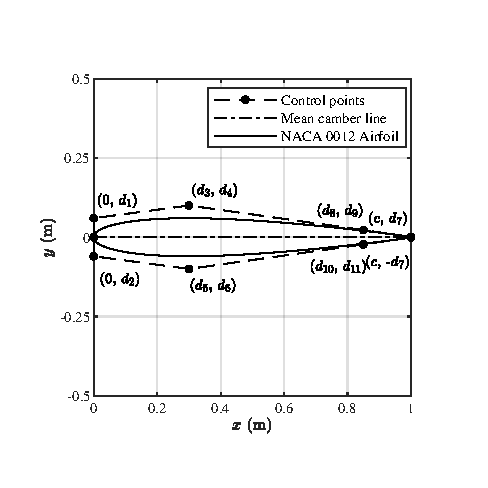
\includegraphics[width=0.7\textwidth]{Figures/Fig20-b.pdf}
\end{figure}
\end{column}

\begin{column}{.5\textwidth}
\begin{figure}[H]
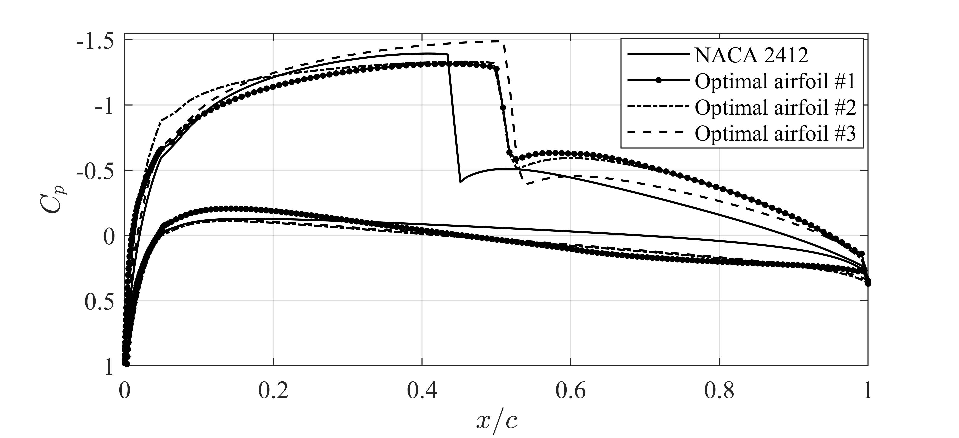
\includegraphics[width=1.1\textwidth]{Figures/Fig23-b.pdf}
\end{figure}
\end{column}
\hfill
\end{columns}
}

\only<3>
{
{\it Derivatives cannot be trusted or evaluated.}
\begin{figure}[H]
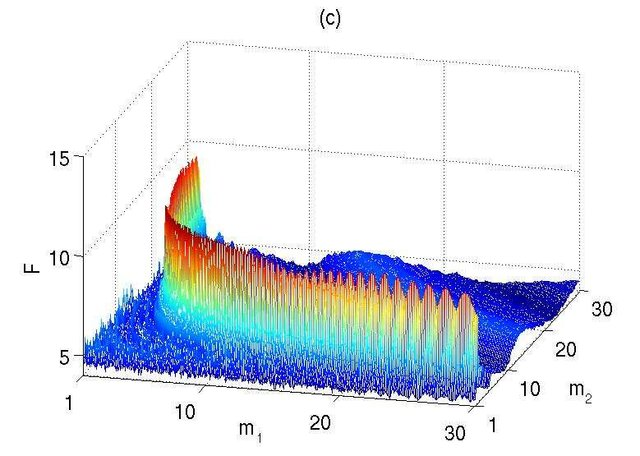
\includegraphics[width=0.4\textwidth]{Figures/noisy.jpeg}
\end{figure}
}

\only<4>
{
{\it BBO challenges}

\begin{figure}[H]
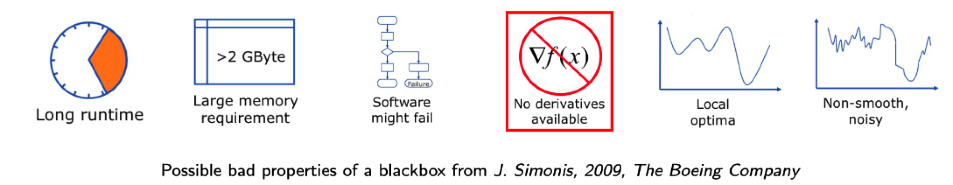
\includegraphics[width=0.9\textwidth]{Figures/BB_challenges.png}
\end{figure}

}
\only<5>
{
{\it John Dennis analogy [Powell 1994]}

\begin{figure}[H]
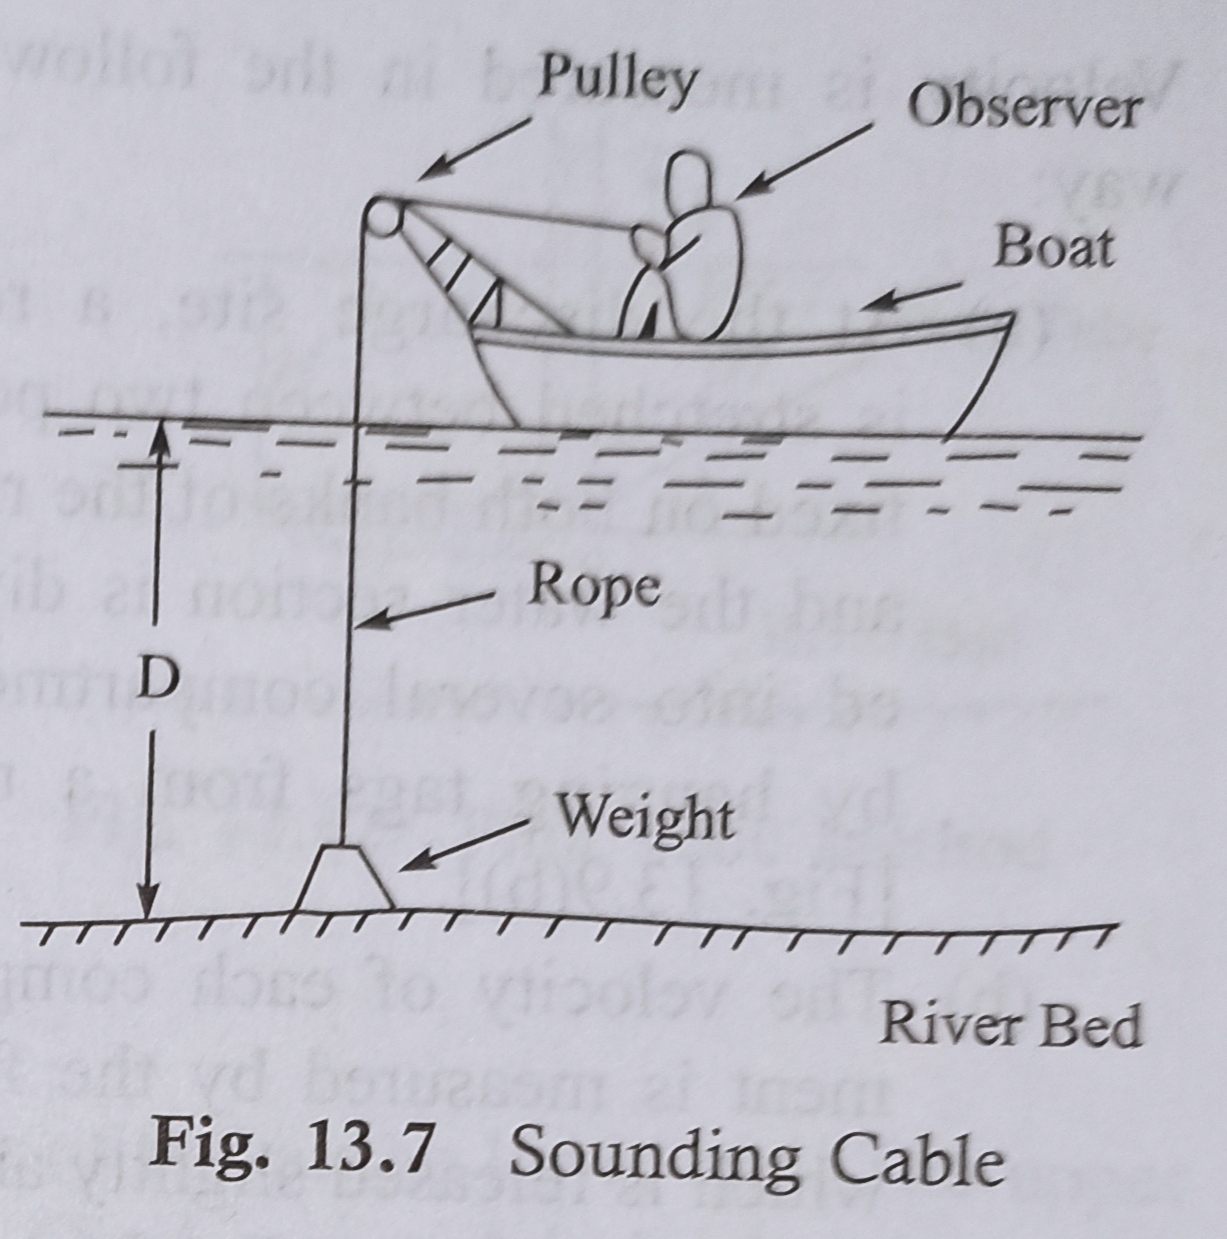
\includegraphics[width=0.35\textwidth]{Figures/fathom.jpeg}
\end{figure}

}
\end{frame}

\begin{frame}{Gradients availablity}
  \begin{figure}[H]
    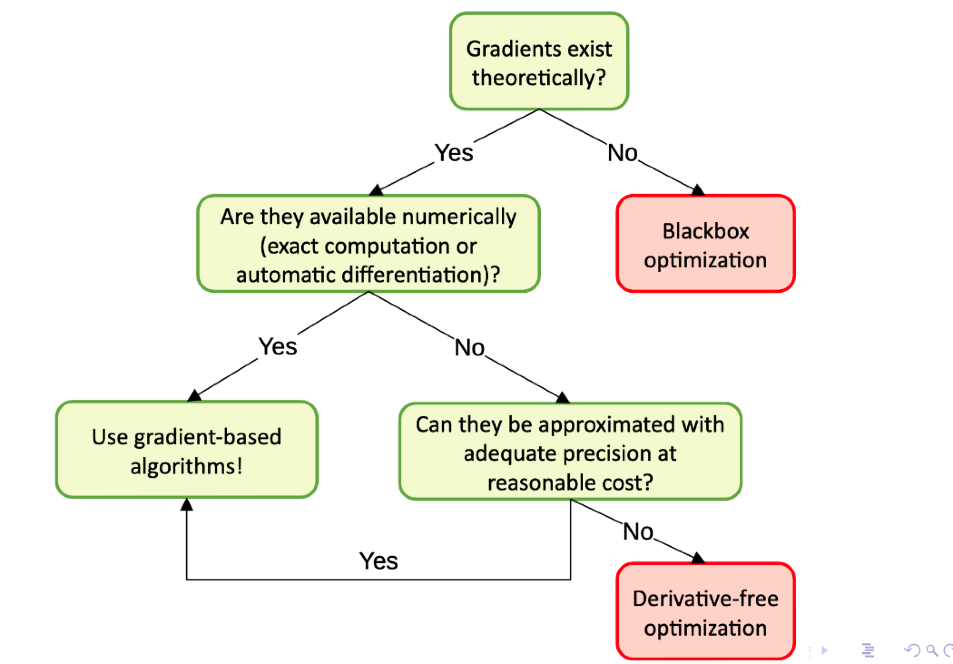
\includegraphics[width=0.95\textwidth]{Figures/GAV.png}
    \end{figure}
\end{frame}

\begin{frame}[t]{Blackbox Optimization Problems} \vspace{4pt}
\begin{block}<1->{Definition: Blackbox optimization}
{\it It refers to problems where objective and constraint functions cannot be exploited.}
\end{block}
\only<1->
{
Often the case when their evaluation requires the execution (usually time-consuming) simulation using computational models, typically inaccessible by the user.
}
\vfill
\begin{block}<2->{Definition: Derivative-free optimization}
{\it It refers to the use of algorithms that utilize only function values because their derivatives are either not defined or not available.}
\end{block}
\only<2>
{
Gradient approximations may sometimes be obtained, but the amount of work required to ensure they are dependable may not be worth the effort.
}
\end{frame}
\begin{frame}{Types of constraints}
The domain: $\Omega= \{x \in X:c_{j}(x) \leq 0, j \in J \} \subset \mathbb{R}^{n}$
\begin{itemize}
  \item The set $X$ represents {\it \color{myblue} unrelaxable constraints}
  \item $c_{j}(x)\leq0$ are {\it \color{myblue} relaxable constraints}
  \item {\it \color{myblue} Hidden constraints}: when the simulation fails for points in $\Omega$
\end{itemize}

\end{frame}

\begin{frame}{Properties of a function}
  \begin{itemize}

    \item
    We consider a function $f: \mathbb{R}^n \rightarrow \mathbb{R}$.
    
    \medskip
    \item
    We define some properties of $f$ {\color{myblue} at $x$}, a point of its domain.
    
    \medskip
    \item
    We say that these properties apply {\color{myblue} near $x$}
    if the property is satisfied on some open neighborhood of $x$.
    
    \medskip
    \item
    We can also consider some properties {\color{myblue} on a domain
    ${\cal X} \subset \mathbb{R}^n$}.
    
    \medskip
    \item
    $f$ is {\color{myblue} continuous} at $x \in \mathbb{R}^n$ if the limit
    $\lim\limits_{y \rightarrow x} f(y)$
    exists and is equal to $f(x)$.
    
    \end{itemize}
\end{frame}

\begin{frame}{Types of variables}
The decision variables $x$ can be any combination of 
\begin{itemize}
  \item Continuous $\mathbb{R}$
  \item Integer $\mathbb{N}$ or $\mathbb{Z}$
  \item binary $\{0,1\}$
  \item granular $\{0,0.05,0.10,...,0.95,1.00\}$
  \item Categorical $\{0,0.05,0.10,...,0.95,1.00\}$
  \begin{itemize}
    \item Ex: Hyper-parameter optimization of deep neural network
  \end{itemize}
\end{itemize}
\begin{figure}[H]
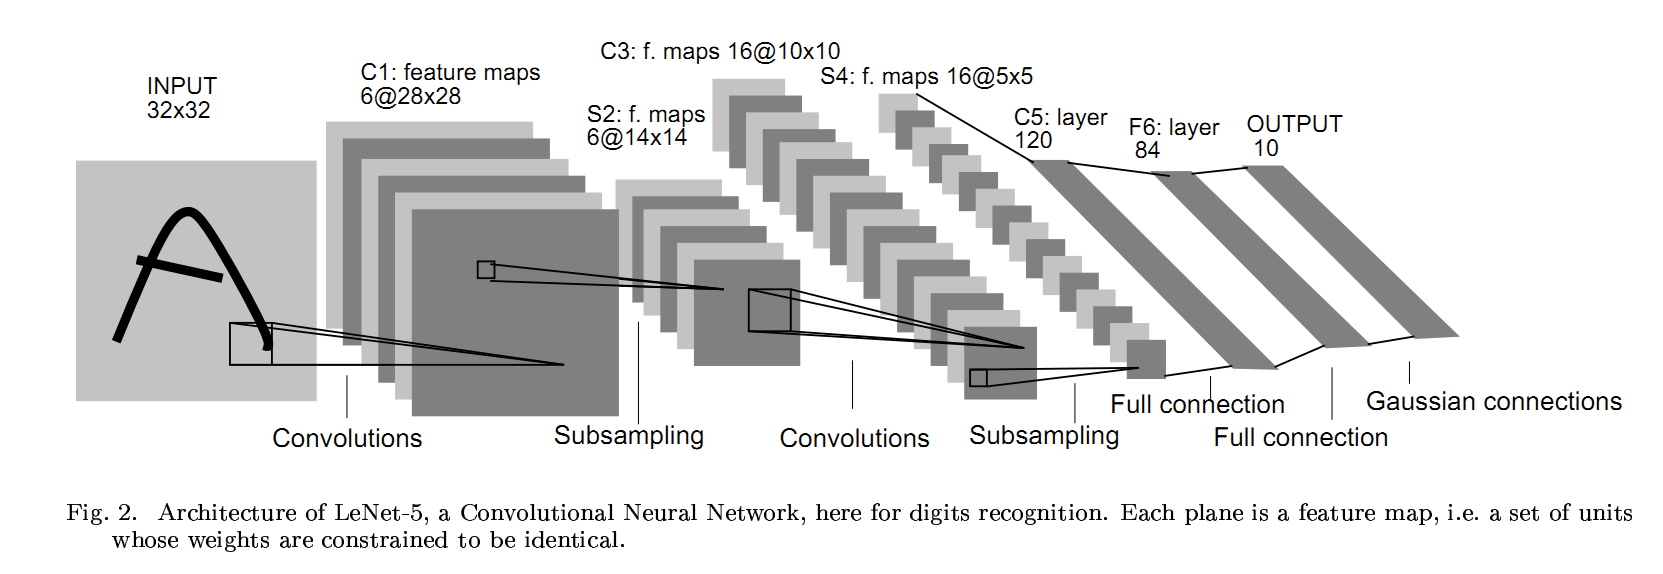
\includegraphics[width=0.8\textwidth]{Figures/CNN.png}
\end{figure}
- No ordinal property\\
- The number of convolution layers impacts the total number of optimization variables
\end{frame}

\begin{frame}{}
  \begin{itemize}
  \item {\transparent{0.2} What is blackbox optimization?}
  \vspace{0.5cm}
  \item {Functions differentiability}
  \vspace{0.5cm}
  \item {\transparent{0.2} Direct search methods}
  \vspace{0.5cm}
  \item {\transparent{0.2} Mesh adaptive direct search method}
  \vspace{0.5cm}
  \item {\transparent{0.2} Implementations}
  \vspace{0.5cm}
  \item {\transparent{0.2} Running example}
  \end{itemize}
\end{frame}

\section{Differentiability}
%--------------------------------------------------------------%
\frame{\frametitle{Differentiability}
%--------------------------------------------------------------%

Consider the function $f: \R^n \rightarrow \R$.

\begin{itemize}

\item
$f$ is {\rd differentiable} at $x \in \R^n$ if there exists $g \in \R^n$ such that
$$\lim\limits_{y \rightarrow x} \frac{f(y)-f(x)-g^{\top}(y-x)}{\| y-x \|}=0 $$

\medskip
\item
If this $g$ exists, it is unique and is called the {\rd gradient} of $f$ at $x$,
denoted ${\rd \nabla f(x)}$.

\medskip
\item
If $f$ is differentiable at $x$, then $f$ is continuous at $x$.

\medskip
\item
{\rd Partial derivatives}:
$$\nabla f(x) = \left( \frac{\partial f(x)}{\partial x_1} , \frac{\partial f(x)}{\partial x_2} , \ldots , \frac{\partial f(x)}{\partial x_n}\right)^{\top} $$

%\medskip
%\item
%All partial derivatives of a function may exist, even if the function is not differentiable.

\end{itemize}

}

%----------------------------------------------------------------------%
\frame{\frametitle{Differentiability classes}
%----------------------------------------------------------------------%
% http://en.wikipedia.org/wiki/Differentiable_function

\begin{itemize}

\item
A function $f:\R^n \rightarrow \R$ is said {\rd of class ${\cal C}^k$},
denoted $f \in {\cal C}^k$, with $0 \leq k \leq \infty$,
if all the possible partial derivatives of the form
$$\frac{\partial^k f} {\partial x_{i_1}\partial x_{i_2}\cdots\partial x_{i_k}}$$
exist and are continuous, where
$i_{\ell} \in \{1, 2, \ldots, n\}$
for all ${\ell} \in \{1, 2, \ldots, k \}$.


\medskip
%
\item
${\cal C}^0$: Continuous functions.

\medskip
%%
\item
${\cal C}^1$: {\rd Continuously differentiable} functions.

\medskip
%%
\item
${\cal C}^\infty$: {\rd Smooth} functions.

\end{itemize}

}

%--------------------------------------------------------------%
\frame{\frametitle{Lipschitz functions}
%--------------------------------------------------------------%

\begin{itemize}

\medskip
\item
$f$ is {\rd Lipschitz} on the set ${\cal X} \subset \R^n$ if there exists a scalar $K>0$ such that
$$|f(x)-f(y)| \leq K \| x-y\| \mbox{ for all } x,y \in {\cal X} $$

\bigskip
\item
$K$ is called the {\rd Lipschitz constant}.


\bigskip


\item
Examples of non-Lipschitz functions:
\begin{itemize}
\item 
$f(x)= \sqrt{x}$ for $x \geq 0$.

\item
Discontinuous functions, $\tan(x)$ for $x \in (-\pi/2,\pi/2)$, $\frac{1}{x}$ for $x \in \mathbb{R}$.

\item
$f(x)= x^2$ for $x \in \mathbb{R}$.
\end{itemize}


Examples of Lipschitz functions:
\begin{itemize}
\item 
$f(x)= \sqrt{x^2 + 5}$ for $x \in \mathbb{R}$, $K=1$.

\item
$\sin(x)$ for $x \in \mathbb{R}$, $K=1$.

\item
$f(x)= \left|x\right|$ for $x \in \mathbb{R}$, $K=1$.
\end{itemize}

\end{itemize}

}

%--------------------------------------------------------------%
\frame{\frametitle{Summary of function types}
%--------------------------------------------------------------%

$f:X \subseteq \R^n \rightarrow \R$ is...

\bigskip

\hspace*{-1cm}
%\begin{center}
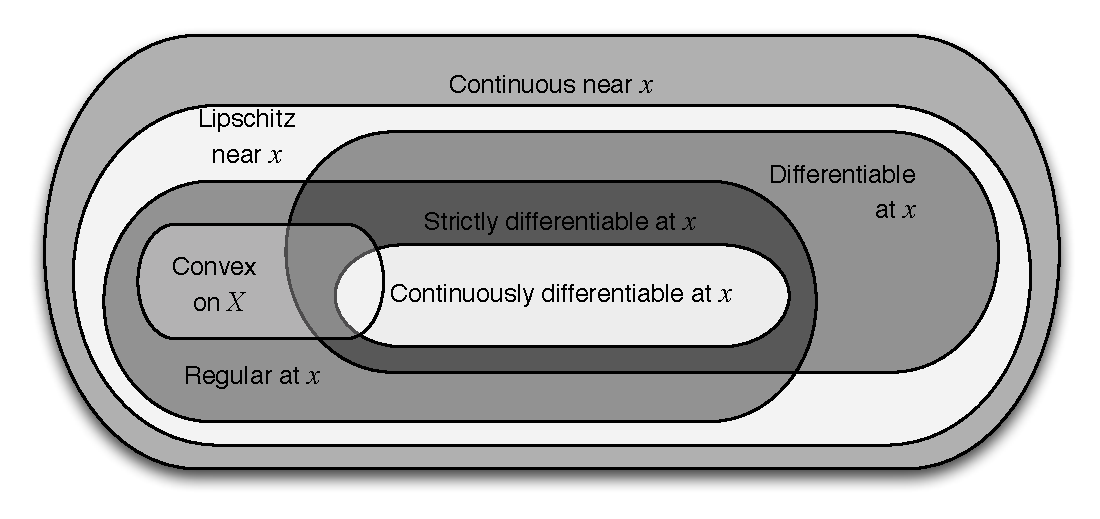
\includegraphics[scale=0.7]{Figures/smooth.pdf}
%\end{center}

}

%------------------------------------------------------------------------------------%
\frame{\frametitle{Convergence analysis (1/2)}
%------------------------------------------------------------------------------------%

\begin{itemize}

\item
An optimization algorithm is not considered {\rd heuristic} when it is backed by
a {\rd convergence analysis} which ensures some properties at the resulting solution $\hat{x}$.

\medskip
\item
This analysis typically depends on some assumptions made about the nature of the problem.
For example: differentiability of $f$, convexity of $\Omega$, etc.

\medskip
\item
Usually, these properties are given as {\rd necessary} or {\rd sufficient} {\rd optimality conditions}.

\medskip
\item
Recall that
{\rd global convergence} refers to 
independence of the starting point.

\end{itemize}
}

%------------------------------------------------------------------------------------%
\frame{\frametitle{Convergence analysis (2/2)}
%------------------------------------------------------------------------------------%

\begin{itemize}

\item
In DFO, we expect global convergence to solutions satisfying some local and necessary optimality conditions, when the
function is supposed Lipschitz.

\medskip
\item
However, a blackbox has no exploitable property and cannot be proven Lipschitz.

\medskip
\item
{\bf But} consider the following choice between two algorithms to apply to such a problem:

\begin{itemize}

\item
Algorithm ${\cal A}$ is a heuristic; it {\bf may} yield a point  $\hat{x}$ where $\nabla f(\hat{x}) \neq 0$ when $f$ is differentiable.

\item
Algorithm ${\cal B}$ guarantees $\nabla f(\hat{x}) =0$ when $f$ is differentiable.

\end{itemize}

The choice is obvious.

\end{itemize}

}

\section{DS methods}
\begin{frame}{General scheme}
  Direct search methods launch the blackbox simulation at tentative trial points in hopes of improving the current best solution.\\
  * The way that the trial points are generated defines the method

  \begin{center}
    \begin{tikzpicture}[
      squarednode1/.style={rectangle, text=white, draw=black!60, fill=black, very thick, minimum height=3em, minimum width=6em},
      squarednode2/.style={rectangle, text=black, draw=black!60, fill=white, very thick, minimum height=3em, minimum width=6em},
      ]
      %Nodes
      \node[squarednode1]      (blackbox)                              {Blackbox};
      \node[squarednode2]      (bottomsquare)       [below=1cm of blackbox] {Algorithm};
  
      %Lines
      \draw[-] (blackbox.east) -- ($(1.85,0)$)
      node [midway, above, draw=none] {$f(x)$}
      node [midway, below, draw=none] {$x\in\Omega?$};
      \draw[->] ($(blackbox.east)+(1,0)$) |- (bottomsquare.east);
      
      \draw[->] ($(bottomsquare.west)+(-1,0)$) |- (blackbox.west);
      \draw[-] (bottomsquare.west) -- ($(-1.85,-1.88)$)
      node [midway, below, draw=none] {$x\in\mathbb{R}^{n}$};
    \end{tikzpicture}
  
  \end{center}
\end{frame}

\begin{frame}{Unconstrained optimization - Coordinate search}
  1952 Fermi and Metropolis\\
  Coordinate Search algorithm.\\

  \begin{columns}[T]
    \begin{column}{0.5\textwidth}
      \begin{center}
      \only<1>{
        \begin{tikzpicture}
        \draw [step=1.0,gray, very thin, xshift=0.5, yshift=-0.5] (0.5,0.5) grid (5.5,3.5);
        \draw[fill=gray] (3.02,2.0) circle (0.08);
        \end{tikzpicture}
      }
      \only<2>{
        \begin{tikzpicture}
          \draw [step=1.0,gray, very thin, xshift=0.5, yshift=-0.5] (0.5,0.5) grid (5.5,3.5);
          % Incumbent solution
          \draw[fill=black] (3.02,2.0) circle (0.08);
          % Polling directions
          \draw[fill=black] (4.02,2.0) circle (0.08);
          \draw[fill=black] (2.02,2.0) circle (0.08);
          \draw[fill=black] (3.02,3.0) circle (0.08);
          \draw[fill=black] (3.02,1.0) circle (0.08);
          % Rectangle
          \draw[draw=black, very thick] (2.02,1.0) rectangle ++(2.0,2.0);
          % Compass
          \draw[black, very thick] (2.02,2.0) -- (4.02,2.0);
          \draw[black, very thick] (3.02,1.0) -- (3.02,3.0);
        \end{tikzpicture}
      }
      \only<3>{
        \begin{tikzpicture}
          \draw [step=1.0,gray, very thin, xshift=0.5, yshift=-0.5] (0.5,0.5) grid (5.5,3.5);
          % Polling directions
          \draw[fill=black] (4.02,2.0) circle (0.08);
          \draw[fill=black] (2.02,2.0) circle (0.08);
          \draw[fill=black] (3.02,3.0) circle (0.08);
          \draw[fill=black] (3.02,1.0) circle (0.08);
          % Rectangle
          \draw[draw=black, very thick] (2.02,1.0) rectangle ++(2.0,2.0);
          % Compass
          \draw[black, very thick] (2.02,2.0) -- (4.02,2.0);
          \draw[black, very thick] (3.02,1.0) -- (3.02,3.0);
          % Incumbent solution
          \draw[fill=green] (3.02,2.0) circle (0.08);
        \end{tikzpicture}
      }
      \only<4>{
        \begin{tikzpicture}
          \draw [step=0.5,gray, very thin, xshift=0.5, yshift=-0.5] (0.5,0.5) grid (5.5,3.5);
          % Polling directions
          \draw[fill=black] (3.52,2.0) circle (0.08);
          \draw[fill=black] (2.52,2.0) circle (0.08);
          \draw[fill=black] (3.02,2.5) circle (0.08);
          \draw[fill=black] (3.02,1.5) circle (0.08);
          % Rectangle
          \draw[draw=black, very thick] (2.52,1.5) rectangle ++(1.0,1.0);
          % Compass
          \draw[black, very thick] (2.52,2.0) -- (3.52,2.0);
          \draw[black, very thick] (3.02,1.5) -- (3.02,2.5);
          % Incumbent solution
          \draw[fill=black] (3.02,2.0) circle (0.08);
        \end{tikzpicture}
      } 
      \only<5>{
        \begin{tikzpicture}
          \draw [step=0.5,gray, very thin, xshift=0.5, yshift=-0.5] (0.5,0.5) grid (5.5,3.5);
          % Polling directions
          \draw[fill=black] (3.02,2.0) circle (0.08);
          \draw[fill=black] (2.52,2.0) circle (0.08);
          \draw[fill=black] (3.02,2.5) circle (0.08);
          \draw[fill=black] (3.02,1.5) circle (0.08);
          % Rectangle
          \draw[draw=black, very thick] (2.52,1.5) rectangle ++(1.0,1.0);
          % Compass
          \draw[black, very thick] (2.52,2.0) -- (3.52,2.0);
          \draw[black, very thick] (3.02,1.5) -- (3.02,2.5);
          % Incumbent solution
          
          \draw[fill=green] (3.52,2.0) circle (0.08);
        \end{tikzpicture}
      } 

      \only<6->{
        \begin{tikzpicture}
          \draw [step=0.5,gray, very thin, xshift=0.5, yshift=-0.5] (0.5,0.5) grid (5.5,3.5);
          % Polling directions
          \draw[fill=black] (4.02,2.0) circle (0.08);
          \draw[fill=black] (3.02,2.0) circle (0.08);
          \draw[fill=black] (3.52,2.5) circle (0.08);
          \draw[fill=black] (3.52,1.5) circle (0.08);
          % Rectangle
          \draw[draw=black, very thick] (3.02,1.5) rectangle ++(1.0,1.0);
          % Compass
          \draw[black, very thick] (3.02,2.0) -- (4.02,2.0);
          \draw[black, very thick] (3.52,1.5) -- (3.52,2.5);
          % Incumbent solution
          \draw[fill=green] (3.52,2.0) circle (0.08);
        \end{tikzpicture}
      } 
      
    \end{center}
    \end{column}
    \begin{column}{0.8\textwidth}
    \only<1>{
      \begin{figure}[H]
        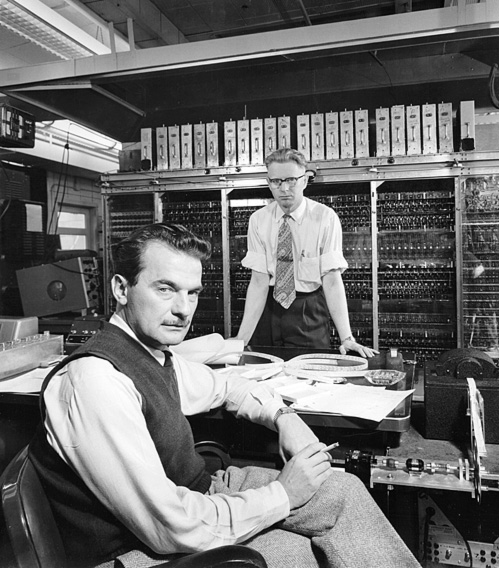
\includegraphics[width=0.5\textwidth]{Figures/maniac.jpeg}\caption*{Metropolis and Richardson in front of the MANIAC computer\\ Source http://www.ominous-valve.com/maniac.html}
      \end{figure}
      }
       \only<2>{
       \begin{itemize}
          \item {\sc Initialization}:\\
            $x_0$ :  starting point in $\mathbbm{R}^n$\\
            $\Delta_0 >0$ :  initial step size
          %
          \medskip
          \item {\sc Poll step}: for $k = 0,1,\ldots$ \\
              if $f(t) < f(x_k)$ for
              $t \in P_k := \{ x_k \pm \Delta_k e_i : i = 1, 2, \ldots, n \}$:\\
                  \hspace*{1cm}
                  $x_{k+1} \leftarrow t$\\
              \hspace*{1cm} $\Delta_{k+1} \leftarrow \Delta_k$  \\
          %
              else (failure): $x_k$ is a local minimum relatively to $P_k$: \\
              \hspace*{1cm}
                    $x_{k+1} \leftarrow x_k$\\
              \hspace*{1cm} $\Delta_{k+1} \leftarrow \Delta_k  / 2$
        \end{itemize}
        }

        \only<3>{
       \begin{itemize}
          \item {\sc Initialization}:\\
            $x_0$ :  starting point in $\mathbbm{R}^n$\\
            $\Delta_0 >0$ :  initial step size
          %
          \medskip
          \item {\sc Poll step}: for $k = 0,1,\ldots$ \\
              if $f(t) < f(x_k)$ for
              $t \in P_k := \{ x_k \pm \Delta_k e_i : i = 1, 2, \ldots, n \}$:\\
                  \hspace*{1cm}
                  $x_{k+1} \leftarrow t$\\
              \hspace*{1cm} $\Delta_{k+1} \leftarrow \Delta_k$  \\
          %
              else (failure): {\color{myblue} $x_k$ is a local minimum relatively to $P_k$}: \\
              \hspace*{1cm}
                    $x_{k+1} \leftarrow x_k$\\
              \hspace*{1cm} $\Delta_{k+1} \leftarrow \Delta_k  / 2$
        \end{itemize}
        }
        \only<4>{
       \begin{itemize}
          \item {\sc Initialization}:\\
            $x_0$ :  starting point in $\mathbbm{R}^n$\\
            $\Delta_0 >0$ :  initial step size
          %
          \medskip
          \item {\sc Poll step}: for $k = 0,1,\ldots$ \\
              if $f(t) < f(x_k)$ for
              $t \in P_k := \{ x_k \pm \Delta_k e_i : i = 1, 2, \ldots, n \}$:\\
                  \hspace*{1cm}
                  $x_{k+1} \leftarrow t$\\
              \hspace*{1cm} $\Delta_{k+1} \leftarrow \Delta_k$  \\
          %
              else (failure): {$x_k$ is a local minimum relatively to $P_k$}: \\
              \hspace*{1cm}
                    {\color{myblue} $x_{k+1} \leftarrow x_k$}\\
              \hspace*{1cm} {\color{myblue}$\Delta_{k+1} \leftarrow \Delta_k  / 2$}
        \end{itemize}
        }
        \only<5>{
       \begin{itemize}
          \item {\sc Initialization}:\\
            $x_0$ :  starting point in $\mathbbm{R}^n$\\
            $\Delta_0 >0$ :  initial step size
          %
          \medskip
          \item {\sc Poll step}: for $k = 0,1,\ldots$ \\
              if {\color{myblue} $f(t) < f(x_k)$} for
              $t \in P_k := \{ x_k \pm \Delta_k e_i : i = 1, 2, \ldots, n \}$:\\
                  \hspace*{1cm}
                  $x_{k+1} \leftarrow t$\\
              \hspace*{1cm} $\Delta_{k+1} \leftarrow \Delta_k$  \\
          %
              else (failure): {$x_k$ is a local minimum relatively to $P_k$}: \\
              \hspace*{1cm}
                    {$x_{k+1} \leftarrow x_k$}\\
              \hspace*{1cm} {$\Delta_{k+1} \leftarrow \Delta_k  / 2$}
        \end{itemize}
        }
        \only<6>{
       \begin{itemize}
          \item {\sc Initialization}:\\
            $x_0$ :  starting point in $\mathbbm{R}^n$\\
            $\Delta_0 >0$ :  initial step size
          %
          \medskip
          \item {\sc Poll step}: for $k = 0,1,\ldots$ \\
              if {$f(t) < f(x_k)$} for
              $t \in P_k := \{ x_k \pm \Delta_k e_i : i = 1, 2, \ldots, n \}$:\\
                  \hspace*{1cm}
                  {\color{myblue} $x_{k+1} \leftarrow t$\\
              \hspace*{1cm} $\Delta_{k+1} \leftarrow \Delta_k$  \\}
          %
              else (failure): {$x_k$ is a local minimum relatively to $P_k$}: \\
              \hspace*{1cm}
                    {$x_{k+1} \leftarrow x_k$}\\
              \hspace*{1cm} {$\Delta_{k+1} \leftarrow \Delta_k  / 2$}
        \end{itemize}
        }
        \only<7>{
       \begin{itemize}
          \item {\sc Initialization}:\\
            $x_0$ :  starting point in $\mathbbm{R}^n$\\
            $\Delta_0 >0$ :  initial step size
          %
          \medskip
          \item {\sc Poll step}: for $k = 0,1,\ldots$ \\
              if {$f(t) < f(x_k)$} for
              $t \in P_k := \{ x_k \pm \Delta_k e_i : i = 1, 2, \ldots, n \}$:\\
                  \hspace*{1cm}
                  { $x_{k+1} \leftarrow t$\\
              \hspace*{1cm} $\Delta_{k+1} \leftarrow \Delta_k$  \\}
          %
              else (failure): {$x_k$ is a local minimum relatively to $P_k$}: \\
              \hspace*{1cm}
                    {$x_{k+1} \leftarrow x_k$}\\
              \hspace*{1cm} {$\Delta_{k+1} \leftarrow \Delta_k  / 2$}
        \end{itemize}
        }

  \end{column}
  \end{columns}
  \only<7>{
    \textbullet\ Remarks
  \begin{itemize}
    \item Evaluation of $x_{0}$ is counted
    \item Extension with bounds: if the algorithm generates a trial point outside of the boundary, then do not evaluate and consider as failure
    \item If the algorithm generates a trial point $x$ found in the cache, then do not evaluate and consider as failure
  \end{itemize}
  }
\end{frame}

\begin{frame}{CS variants}
  \begin{figure}[H]
    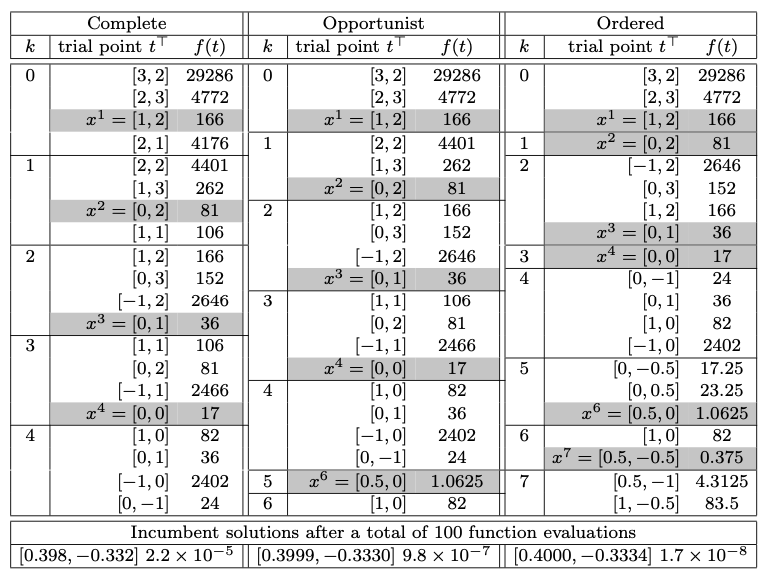
\includegraphics[width=0.8\textwidth]{Figures/CS_variants.png}
  \end{figure} 
\end{frame}

\begin{frame}{CS evolution}
  
  \begin{columns}[T]
    \begin{column}{0.5\textwidth}
      1961 Hooke and Jeeves - Pattern Search\\
      1997 Torczon - Genaralized Pattern Search
      \begin{center}
      \only<1>
      {
        \begin{tikzpicture}
          \draw [step=1.0,gray, very thin, xshift=0.5, yshift=-0.5] (0.5,0.5) grid (5.5,3.5);
          % Incumbent solution
          \draw[fill=black] (3.02,2.0) circle (0.08);
          % Polling directions
          \draw[fill=black] (4.02,3.0) circle (0.08);
          \draw[fill=black] (4.02,1.0) circle (0.08);
          \draw[fill=black] (2.02,3.0) circle (0.08);
          \draw[fill=black] (2.02,1.0) circle (0.08);
          % Rectangle
          \draw[draw=black, very thick] (2.02,1.0) rectangle ++(2.0,2.0);
          % Compass
          \draw[black, very thick] (2.02,1.0) -- (4.02,3.0);
          \draw[black, very thick] (2.02,3.0) -- (4.02,1.0);
        \end{tikzpicture}
      }
      \only<2>{
        \begin{tikzpicture}
          \draw [step=0.5,gray, very thin, xshift=0.5, yshift=-0.5] (0.5,0.5) grid (5.5,3.5);
          % Polling directions
          \draw[fill=black] (3.52,2.0) circle (0.08);
          \draw[fill=black] (2.52,1.5) circle (0.08);
          \draw[fill=black] (2.52,2.5) circle (0.08);
          % Rectangle
          \draw[draw=black, very thick] (2.52,1.5) rectangle ++(1.0,1.0);
          % Compass
          \draw[black, very thick] (3.02,2.0) -- (3.52,2.0);
          \draw[black, very thick] (3.02,2.0) -- (2.52,1.5);
          \draw[black, very thick] (3.02,2.0) -- (2.52,2.5);
          % Incumbent solution
          \draw[fill=black] (3.02,2.0) circle (0.08);
        \end{tikzpicture}
      } 
      \only<3->{
        \begin{tikzpicture}
          \draw [step=0.5,gray, very thin, xshift=0.5, yshift=-0.5] (0.5,0.5) grid (5.5,3.5);
          % Polling directions
          \draw[fill=black] (3.52,2.0) circle (0.08);
          \draw[fill=black] (2.52,1.5) circle (0.08);
          \draw[fill=black] (2.52,2.5) circle (0.08);
          \draw[fill=blue] (4.52,1.5) circle (0.08);
          \draw[fill=blue] (1.02,2.5) circle (0.08);
          % Rectangle
          \draw[draw=black, very thick] (2.52,1.5) rectangle ++(1.0,1.0);
          % Compass
          \draw[black, very thick] (3.02,2.0) -- (3.52,2.0);
          \draw[black, very thick] (3.02,2.0) -- (2.52,1.5);
          \draw[black, very thick] (3.02,2.0) -- (2.52,2.5);
          % Incumbent solution
          \draw[fill=black] (3.02,2.0) circle (0.08);
        \end{tikzpicture}
      } 


    \end{center}
    \end{column}
    \begin{column}{0.8\textwidth}
      \only<1>{Mesh coarsens on successful iterations}
      \only<2>{Mesh refines on unsuccessful iterations}
      \only<3->{
        \begin{center}
          \begin{tikzpicture}[
            squarednode1/.style={rectangle, text=white, draw=black!60, fill=black, very thick, minimum height=3em, minimum width=6em},
            squarednode2/.style={rectangle, text=black, draw=black!60, fill=white, very thick, minimum height=3em, minimum width=6em, align=center},
            ]
            %Nodes
            \node[squarednode1]      (blackbox)                              {Blackbox};
            \node[squarednode2]      (bottomsquare)       [below=1cm of blackbox] {GPS\\ {\color{blue}Search step}\\ {\color{red}Poll step}};
        
            %Lines
            \draw[-] (blackbox.east) -- ($(1.85,0)$)
            node [midway, above, draw=none] {$f(x)$}
            node [midway, below, draw=none] {$x\in\Omega?$};
            \draw[->] ($(blackbox.east)+(1,0)$) |- (bottomsquare.east);
            
            \draw[->] ($(bottomsquare.west)+(-1,0)$) |- (blackbox.west);
            \draw[-] (bottomsquare.west) -- ($(-1.85,-2.)$)
            node [midway, below, draw=none] {$x\in\mathbb{R}^{n}$};
          \end{tikzpicture}
        \end{center}
      }
    \end{column}
  \end{columns}
  \begin{block}<4>{Theorm (Convergence analysis 2003 - Clark calculus)}
    {\it Let $\hat{x}$ be an accumlation point of the sequence of mesh local optimizers on meshes that get infinitely fine.\\
    If $f$ is Lipshitz near $\hat{x}$, then $f^{\circ}(\hat{x};d)\geq 0$ for all directions $d$ used infinitely often.\\
    The set of such directions forms a positive basis for $\mathbb{R}^{n}$}
  \end{block}
  
\end{frame}


\begin{frame}{}
  \begin{columns}[T]
    \begin{column}{.6\textwidth}
      \vspace*{-.25cm}
  \begin{figure}[ht]
    \begin{center}
     % \fbox{
        \begin{small}
          \begin{minipage}{4in}
            \vspace*{5pt}
            {\begin{large} \textbf{[0] Initializations}   \end{large}} ($x_0$, $\Delta_0$ ) \\
              \begin{large}  \textbf{[1] Iteration $k$}  \end{large} \\
              \hspace*{1cm}
              \begin{tabular}{|l}
                   {{\bf [1.1] (global) Search}}  \\
                     \hspace*{1cm}
                     \begin{tabular}{|l}
                       select a finite number of mesh points \\
                       sort these points \\
                       evaluate candidates opportunistically \\
                     \end{tabular} \\
                   {{\bf [1.2] (local) Poll} (if the Search failed)} \\
                   \hspace*{1cm}
                     \begin{tabular}{|l}
                                    construct poll set $P_k=\{ x_k + \Delta_k d : d \in D_k \}$ \\
                                    sort($P_k$) \\
                                    evaluate candidates opportunistically \\
                     \end{tabular}
              \end{tabular} \\
             \begin{large}  \textbf{[2] Updates}  \end{large} \\
             \hspace*{1cm}
                     \begin{tabular}{|l}
                           if success \\
                                        \hspace*{1cm}
                                        \begin{tabular}{|l}
                                           $x_{k+1} \leftarrow $ success point \\
                                           possibly increase $\Delta_k$ \\
                                       \end{tabular}      \\
                          else  \\
                                        \hspace*{1cm}
                                        \begin{tabular}{|l}
                                           $x_{k+1} \leftarrow x_k$ \\
                                           decrease $\Delta_k$ \\
                                       \end{tabular}      \\         
	                    $k    \leftarrow     k+1$, stop or go to {\bf [1]} \\
                     \end{tabular}
          \end{minipage}
        \end{small}
    %   }
      \end{center}
    \end{figure}
    \end{column}
    \begin{column}{.4\textwidth}
      \begin{center}
        \begin{tikzpicture}[
          squarednode1/.style={rectangle, text=white, draw=black!60, fill=black, very thick, minimum height=3em, minimum width=6em},
          squarednode2/.style={rectangle, text=black, draw=black!60, fill=white, very thick, minimum height=3em, minimum width=6em, align=center},
          ]
          %Nodes
          \node[squarednode1]      (blackbox)                              {Blackbox};
          \node[squarednode2]      (bottomsquare)       [below=1cm of blackbox] {GPS\\ {\color{blue}Search step}\\ {\color{red}Poll step}};
      
          %Lines
          \draw[-] (blackbox.east) -- ($(1.85,0)$)
          node [midway, above, draw=none] {$f(x)$}
          node [midway, below, draw=none] {$x\in\Omega?$};
          \draw[->] ($(blackbox.east)+(1,0)$) |- (bottomsquare.east);
          
          \draw[->] ($(bottomsquare.west)+(-1,0)$) |- (blackbox.west);
          \draw[-] (bottomsquare.west) -- ($(-1.85,-2.)$)
          node [midway, below, draw=none] {$x\in\mathbb{R}^{n}$};
        \end{tikzpicture}
      \end{center}
    \end{column}
  \end{columns}
\end{frame}

%---------------------------------------------------------------------------------%
\frame{\frametitle{GPS: Example of poll directions}
%---------------------------------------------------------------------------------%

 $P_k = \{ x_k + \Delta_k d: d \in D_k \}$; $n+1$ mesh points
at distance $\Delta_k$ from $x_k$

%--------------------------------------------------------------------------
\begin{figure}[ht]
\setlength{\unitlength}{0.6mm}
 \begin{picture}(34,43)(3,0)
   \put(20,41){\makebox(0,0){${\Delta_k = 1}$}}

   \multiput(4,4)(0,16){3}
   {
     \put(0,0){\line(1,0){32}}
   }
   \multiput(4,4)(16,0){3}
   {
     \put(0,0){\line(0,1){32}}
   }

   \put(20,20){\circle*{.9}}
   \put(23,18){\makebox(0,0){$_{x_k}$}}


   \thicklines
   \put(3.9,3.9){\line(1,0){32.2}}
   \put(3.9,3.9){\line(0,1){32.2}}
   \put(36.1,36.1){\line(-1,0){32.2}}
   \put(36.1,36.1){\line(0,-1){32.2}}

   \put(4,4.1){\line(1,0){32}}
   \put(4.1,4){\line(0,1){32}}
   \put(36,35.9){\line(-1,0){32}}
   \put(35.9,36){\line(0,-1){32}}
 
 \textcolor{myblue}{
   \put(20,20){\line(1,1){16}}
   \put(20,20){\line(-1,0){16}}
   \put(20,20){\line(0,-1){16}}
   \put(36,36){\circle*{.9}}
   \put(35,38){\makebox(0,0){$_{p^1}$}}
   \put(4,20){\circle*{.9}}
   \put(6.5,18){\makebox(0,0){$_{p^2}$}}
   \put(20,4){\circle*{.9}}
   \put(20,1){\makebox(0,0){$_{p^3}$}}}

 \end{picture}
 %
 %
 %
 \begin{picture}(34,43)(3,0)
   \put(20,41){\makebox(0,0){${\Delta_{k+1}= \frac{1}{2}}$}}

   \multiput(4,4)(0,8){5}
   { \put(0,0){\line(1,0){32}} }
   \multiput(4,4)(8,0){5}
   { \put(0,0){\line(0,1){32}} }

   \put(20,20){\circle*{.9}}
   \put(17,18.5){\makebox(0,0){$_{x_{k+1}}$}}

   \thicklines
   \put(11.9,11.9){\line(1,0){16.2}}
   \put(11.9,11.9){\line(0,1){16.2}}
   \put(28.1,28.1){\line(-1,0){16.2}}
   \put(28.1,28.1){\line(0,-1){16.2}}

   \put(12,12.1){\line(1,0){16}}
   \put(12.1,12){\line(0,1){16}}
   \put(28,27.9){\line(-1,0){16}}
   \put(27.9,28){\line(0,-1){16}}
 
 \textcolor{myblue}{
   \put(20,20){\line(1,-1){8}}
   \put(20,20){\line(-1,0){8}}
   \put(20,20){\line(0,1){8}}
   \put(28,12){\circle*{.9}}
   \put(31,10){\makebox(0,0){$_{p^4}$}}
   \put(12,20){\circle*{.9}}
   \put(10,21.5){\makebox(0,0){$_{p^6}$}}
   \put(20,28){\circle*{.9}}
   \put(22,31){\makebox(0,0){$_{p^5}$}}}

\end{picture}


\begin{picture}(34,43)(3,0)
  \put(20,41){\makebox(0,0){$\Delta_{k+2}= \frac{1}{4}$}}

  \multiput(4,4)(0,4){9}
  { \put(0,0){\line(1,0){32}} }
  \multiput(4,4)(4,0){9}
  { \put(0,0){\line(0,1){32}} }

  \put(20,20){\circle*{.9}}
  \put(20,18){\makebox(0,0){$_{x_{k+2}}$}}
  \thicklines
  \put(15.9,15.9){\line(1,0){8.2}}
  \put(15.9,15.9){\line(0,1){8.2}}
  \put(24.1,24.1){\line(-1,0){8.2}}
  \put(24.1,24.1){\line(0,-1){8.2}}
  \put(16,16.1){\line(1,0){8}}
  \put(16.1,16){\line(0,1){8}}
  \put(24,23.9){\line(-1,0){8}}
  \put(23.9,24){\line(0,-1){8}}

\textcolor{myblue}{
  \put(20,20){\line(1,1){4}}
  \put(20,20){\line(-1,0){4}}
  \put(20,20){\line(1,-1){4}}
  \put(24,24){\circle*{.9}}
  \put(23,26){\makebox(0,0){$_{p^7}$}}
  \put(16,20){\circle*{.9}}
  \put(14,21){\makebox(0,0){$_{p^8}$}}
  \put(24,16){\circle*{.9}}
  \put(22,14){\makebox(0,0){$_{p^9}$}}}
  \put(-15,-4){\makebox(0,0){14 different ways of defining $D_k$ on this mesh}}

\end{picture}

\end{figure}
}

\begin{frame}{}
  \begin{itemize}
  \item {\transparent{0.2} What is blackbox optimization?}
  \vspace{0.5cm}
  \item {\transparent{0.2} Functions differentiability}
  \vspace{0.5cm}
  \item {\transparent{0.2} Direct search methods}
  \vspace{0.5cm}
  \item {Mesh adaptive direct search method}
  \vspace{0.5cm}
  \item {\transparent{0.2} Implementations}
  \vspace{0.5cm}
  \item {\transparent{0.2} Running example}
  \end{itemize}
\end{frame}



\section{MADS}
\begin{frame}{The MADS algorithm}
  \begin{algorithm}[H]
    \begin{algorithmic}[1]
      \STATE{Initialization}\\
      \hspace{1em} $x^{0} \in \R^{n}$ \hspace{3em} initial point\\
      \hspace{1em} $\Delta^{0} \in (0, \infty)$ \hspace{1.7em} initial frame size parameter
  
      \STATE{Parameter Update}\\
      \hspace{1em} set the mesh size parameter to $\delta^{k}\leq \Delta^{k}$\\
      \hspace{1em} define the mesh $M^{k}$
  
      \STATE{``Optional'' global {\rd Search} on mesh $M^{k}$}\\
      \hspace{1em} if $f(t)<f(x^{k})$ for some $t$ in a finite subset of the mesh $M^{k}$\\
      \hspace{3.5em} set $x^{k+1} \leftarrow t$ and $\Delta^{k+1} \leftarrow 2\Delta^{k}$ and go to Step 5.
  
      \STATE{Local {\rd Poll} on Mesh $M^{k}$}\\
      \hspace{1em} select a positive spanning set $D^{k}_{\Delta}$\\
      \hspace{1em} if $f(t)<f(x^{k})$ for some $t \in P^{k}=\{x^{k}+\delta^{k}d:d\in D^{k}_{\Delta}\}$ in a finite subset of the mesh $M^{k}$\\
      \hspace{3.5em} set $x^{k+1} \leftarrow t$ and $\Delta^{k+1} \leftarrow 2\Delta^{k}$\\
      \hspace{1em} else \hspace{0.5em} set $x^{k+1} \leftarrow x^{k}$ and $\Delta^{k+1} \leftarrow \frac{1}{2}\Delta^{k}$
      \STATE{Termination check}\\
      otherwise $k \leftarrow k+1$ and return to Step 2.
    \end{algorithmic}
    \caption*{MADS main algorithm}
    \label{alg:seq}
    \end{algorithm}
\end{frame}

\begin{frame}{MADS algorithm workflow}
  \begin{center}
    \begin{figure}[H]
    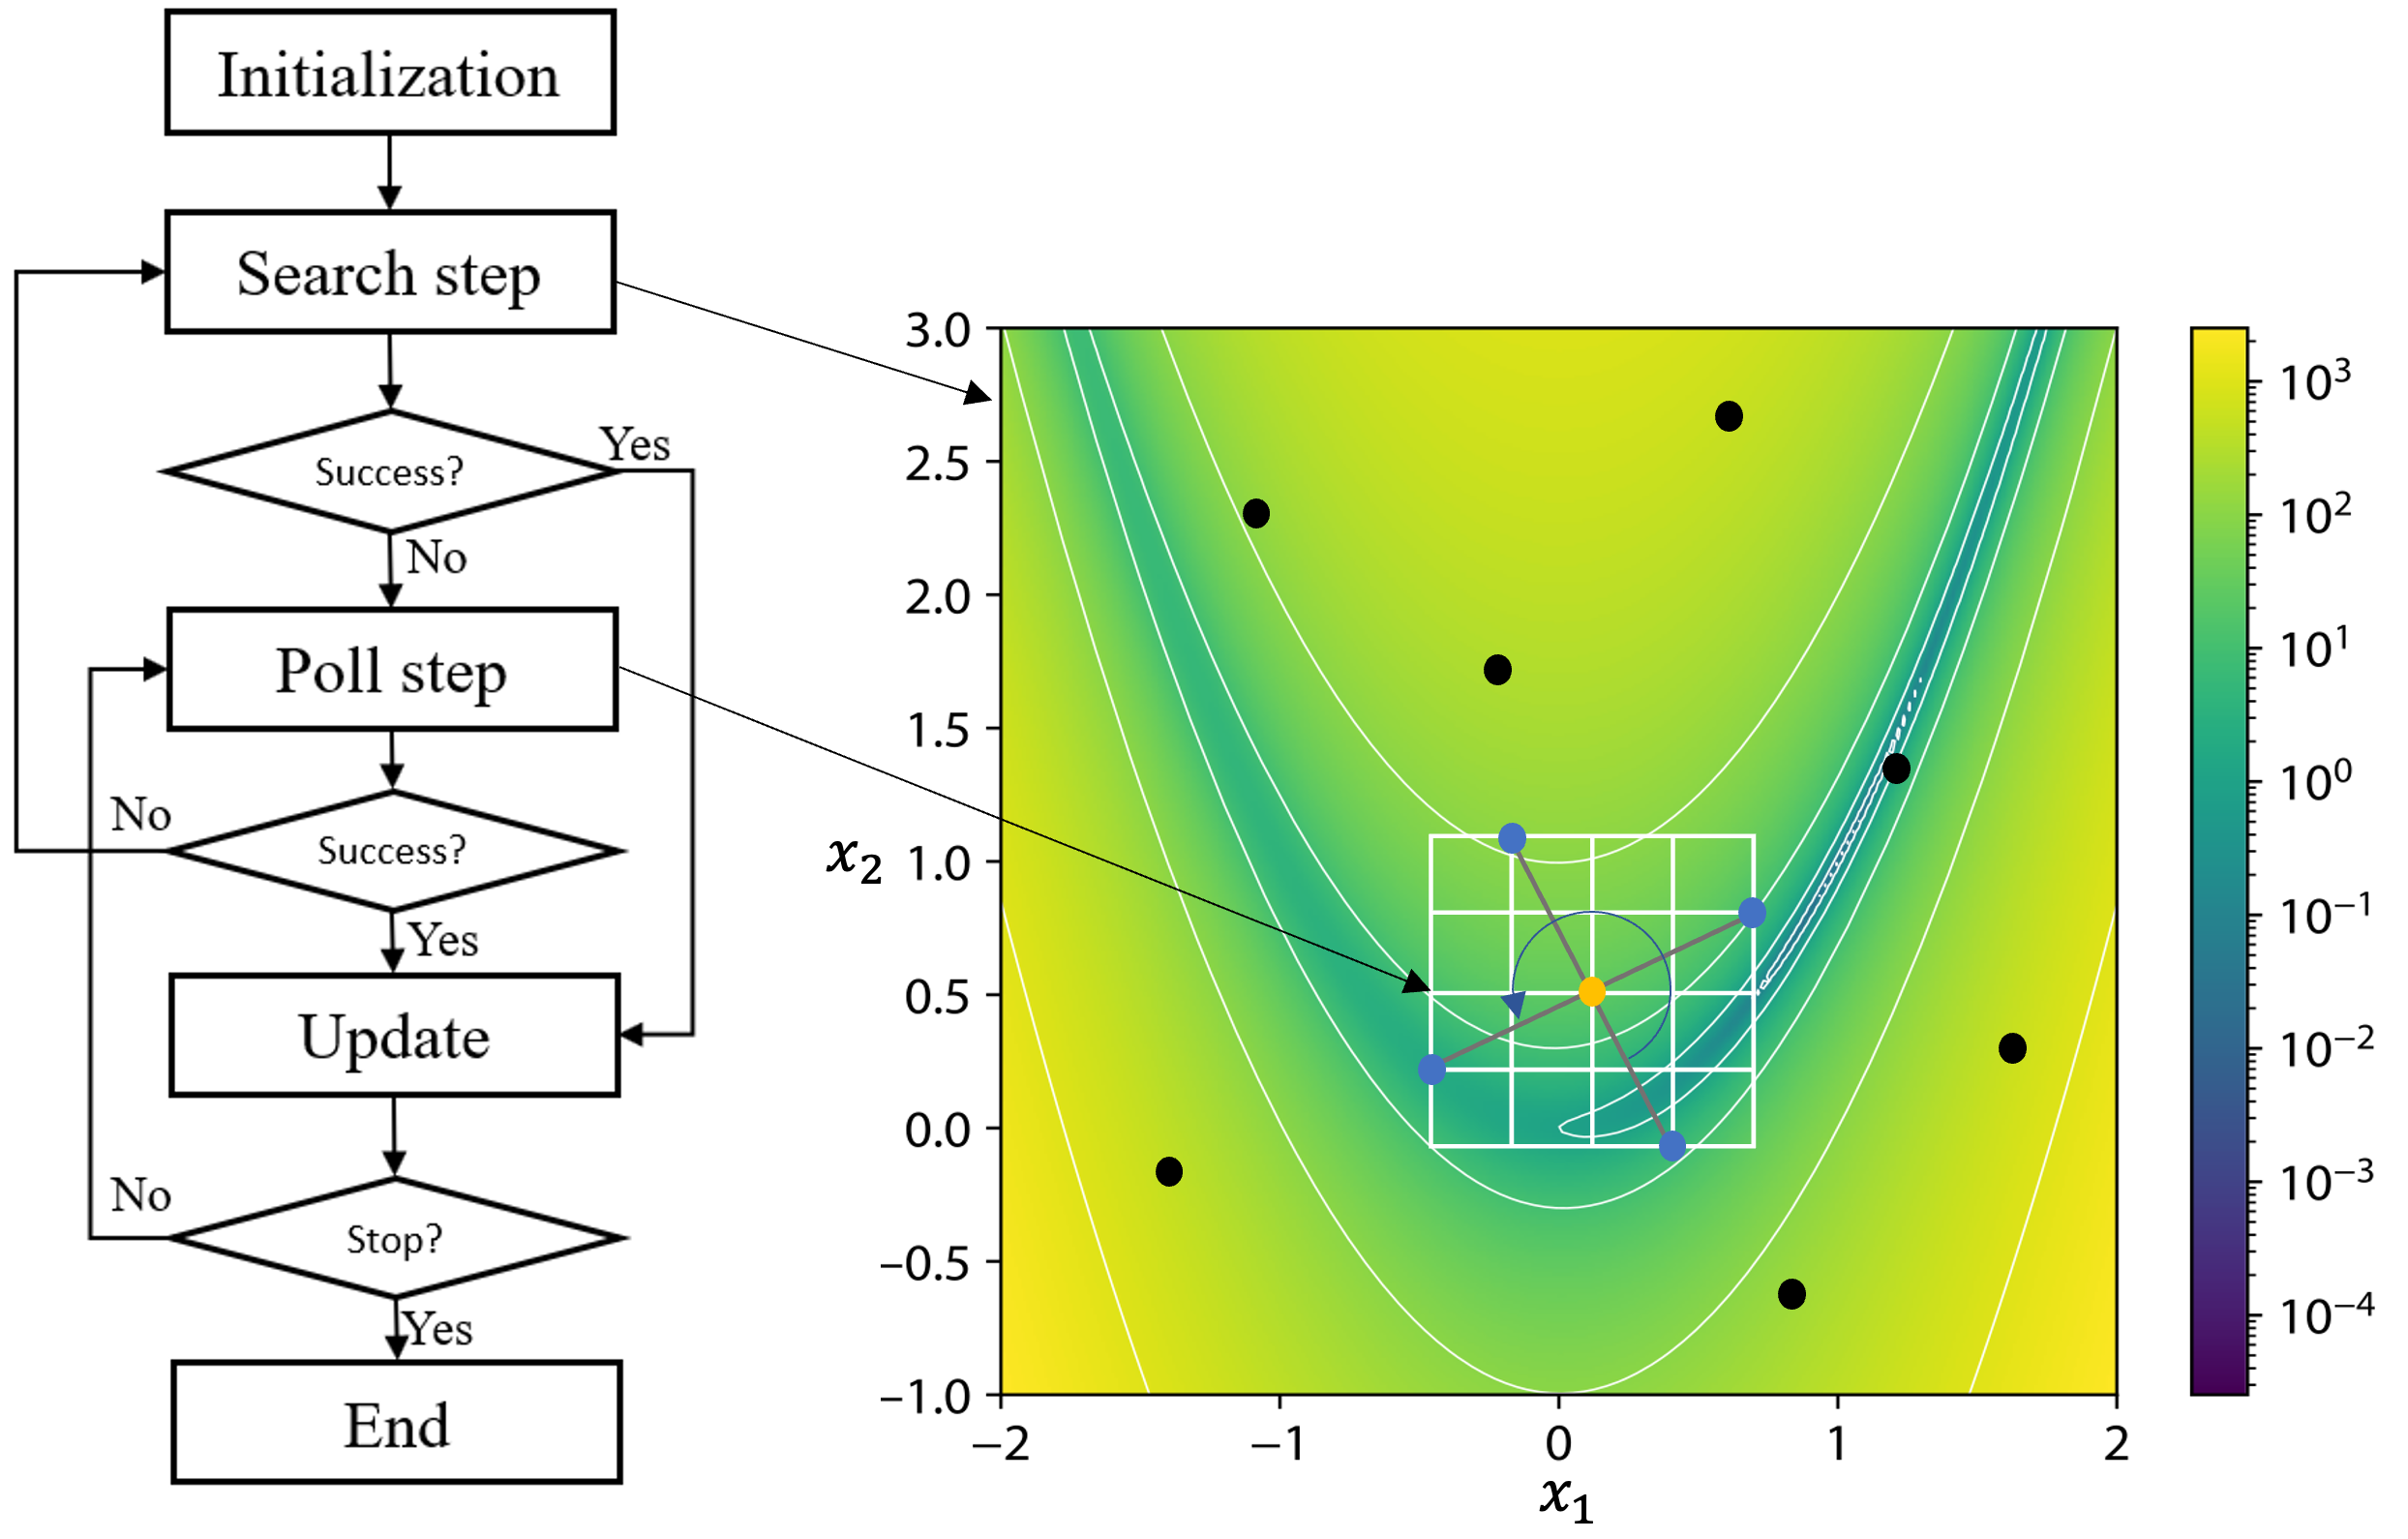
\includegraphics[width=0.9\textwidth]
    {Figures/flow-chart.png}
    \end{figure}
    \end{center}
\end{frame}

\begin{frame}{Mesh and frame definitions}

  \begin{center}
    \begin{figure}[H]
    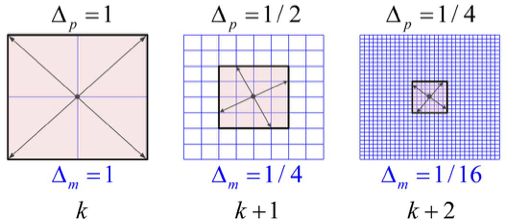
\includegraphics[width=0.5\textwidth]
    {Figures/Poll-Mesh.png}
    \end{figure}
  \end{center}

  \begin{block}<1->{Definition: Mesh and Mesh Size Parameter}
    {\it Let $G \in \mathbb{R}^{n\times n}$ be an invertible matrix and the columns of $Z \in \mathbb{Z}^{n \times p}$ form a positive spanning set for $\mathbb{R}^n$. Define $D = GZ$. The mesh of coarseness $\delta^{k} > 0$ generated by $D$, centered at the incumbent solution $x_{k} \in \mathbb{R}^n$, is defined by
    $M^{k} := \{ x^{k} + \delta^{k}D_{y} : y \in \mathbb{N}^{p} \subset \mathbb{R}^{n}, \}$
    where $\delta^{k}$ is called the mesh size parameter.}
  \end{block}

  \begin{block}<1->{Definition: Frame and Frame Size Parameter}
    {\it Let $G \in \mathbb{R}^{n\times n}$ be an invertible matrix and the columns of $Z \in \mathbb{Z}^{n \times p}$ form a positive spanning set for $\mathbb{R}^n$. Define $D = GZ$. Select a mesh size parameter $\delta^{k} > 0$ and let $\Delta^{k}$ be such that $\delta^{k} \leq \Delta^{k}$. The frame of extent $\Delta^{k}$ generated by $D$, centered at the incumbent solution $x_{k} \in \mathbb{R}^n$, is defined by
    $F^{k} := \{ x \in M^{k} : ||x-x^{k}||_{\infty} \leq \Delta^{k}b \}$
    with $b = \text{max}\{ ||d^{\prime}||_{\infty} : d^{\prime} \in \mathbb{D} \}$ and $\Delta^{k}$ is called the frame size parameter.}
  \end{block}
\end{frame}

\begin{frame}{Dense (rich) set of polling directions}
  \begin{center}
    \begin{figure}[H]
    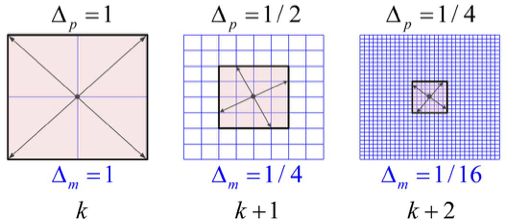
\includegraphics[width=0.5\textwidth]
    {Figures/Poll-Mesh.png}
    \end{figure}
  \end{center}

  \begin{block}<1->{Definition: Asymptotically Dense}
    {\it The set $V \subseteq \mathbb{R}^{n}$ is said to be asymptotically dense if the normalised $set \{v/||v||:v \in V\}$ is dense on the {\rd unit sphere} $S=\{w\in \mathbb{R}^{n} :|w|= 1\}$.}
  \end{block}

  \begin{block}<1->{Definition: Householder Matrix}
    {\it Let $V \subseteq \mathbb{R}^{n}$ be a {\rd normalized vector}. The Householder matrix H associated with $v$ is $H:=I-2vv^{T} \in \mathbb{R}^{n \times n}$, where I is the $n \times n$ {\rd identity matrix}.}
  \end{block}
\end{frame}

\begin{frame}{}
  \begin{itemize}
  \item {\transparent{0.2} What is blackbox optimization?}
  \vspace{0.5cm}
  \item {\transparent{0.2} Functions differentiability}
  \vspace{0.5cm}
  \item {\transparent{0.2} Direct search methods}
  \vspace{0.5cm}
  \item {\transparent{0.2} Mesh adaptive direct search method}
  \vspace{0.5cm}
  \item {Implementations}
  \vspace{0.5cm}
  \item {\transparent{0.2} Running example}
  \end{itemize}
\end{frame}

\section{implementations}
%-------------------------------------%
\frame{\frametitle{MADS implementations (1/2)} 
%-------------------------------------%

\begin{itemize}

\item
MADS is a general framework. It defines  the conditions on the directions,
but do not define the direction themselves

\medskip
\item
There are several implementations:

\begin{itemize}

\medskip
\item
{\rd LT-MADS:} Based on Lower-Triangular random matrices%~\cite{AuDe2006}

\medskip
\item
{\rd QR-MADS:} Based on the QR decomposition and on normally distributed directions~%\cite{VDAs2013}

\medskip
\item
{\rd OrthoMADS:} Quasi-random, deterministic, and orthogonal directions.
Current default in {\sf NOMAD}~%\cite{AbAuDeLe09}

\end{itemize}

\end{itemize}

}

%-------------------------------------%
\frame{\frametitle{MADS implementations (2/2)} 
%-------------------------------------%

\begin{itemize}

\item
Several programs that implement MADS are available:

\begin{itemize}

\medskip
\item
{\rd MATLAB:} \texttt{NOMADm}: \href{https://github.com/khbalhandawi/MECH559_notebooks/blob/master/MATLAB_Algorithms/NomadM/nomadm.m}{https://github.com/khbalhandawi/MECH559\_notebooks/\allowbreak blob/master/MATLAB\_Algorithms/NomadM/nomadm.m}

\medskip
\item
{\rd Python:} \texttt{OMADS}: \href{https://ahmed-bayoumy.github.io/OMADS/}{https://ahmed-bayoumy.github.io/OMADS/}

\medskip
\item
{\rd C++ (with interfaces to various languages):} \texttt{NOMAD}: \href{https://nomad-4-user-guide.readthedocs.io/en/latest/index.html}{https://nomad-4-user-guide.readthedocs.io/en/latest/index.html}\\
This implements the state-of-the-art in MADS development.

\end{itemize}

\end{itemize}

}

\begin{frame}{}
  \begin{itemize}
  \item {\transparent{0.2} What is blackbox optimization?}
  \vspace{0.5cm}
  \item {\transparent{0.2} Functions differentiability}
  \vspace{0.5cm}
  \item {\transparent{0.2} Direct search methods}
  \vspace{0.5cm}
  \item {\transparent{0.2} Mesh adaptive direct search method}
  \vspace{0.5cm}
  \item {\transparent{0.2} Implementations}
  \vspace{0.5cm}
  \item {Running example}
  \end{itemize}
\end{frame}

\end{document}